\chapter{Approximate Bayesian methods}\label{chap15}

\section*{Solutions of Exercises}\label{sec11_1}
\begin{enumerate}[leftmargin=*]

\item \textbf{g-and-k distribution for financial returns continues}

Simulate a dataset following the specification given in the g-and-k distribution for financial returns example. Set $\theta_1 = 0.8$, $a = 1$, $b = 0.5$, $g = -1$, and $k = 1$, with a sample size of 500, and use the same prior as in this example. Implement the ABC accept/reject algorithm from scratch using one million prior draws, selecting the 1,000 draws with the smallest distance.\footnote{Note that this setting does not satisfy the asymptotic requirements for Bayesian consistency. However, it serves as a pedagogical exercise.}

\begin{itemize}
	\item Perform a linear regression adjustment using the posterior draws of our ABC-AR algorithm (ABC-AR-Adj).
	\item Compare the results with those obtained using the ABC-AR implementation in the \textit{EasyABC} package, ensuring that the computational time is relatively similar between both implementations.
	\item Compare the posterior results of ABC-AR, ABC-AR-Adj and EasyABC with the population values.
\end{itemize}

\textbf{Answer:}

The following code implements our ABC-AR algorithm, following the steps outlined in the ABC-AR Algorithm of the book. Users can observe that a linear regression adjustment is applied; however, due to multicollinearity issues, one summary statistic is omitted in the prediction step (see the \textit{abc} package for alternative regression adjustments).  

Figure \ref{figABCown} presents the posterior distributions of $\theta_1$, $g$, and $k$ using both our ABC implementations and the \textit{EasyABC} package. We observe that our algorithms provide less information about $\theta_1$ compared to the \textit{EasyABC} implementation. Conversely, our algorithms offer more information about $g$ and $k$ than the \textit{EasyABC} function. Additionally, regression adjustment helps center the posterior distributions of $g$ and $k$ around the population parameters. But, this is no the case regarding $\theta_1$. Moreover, applying regression adjustment introduces a degree of smoothness to the distributions. Overall, in all implementations, the 95\% credible intervals encompass the population values.

\begin{tcolorbox}[enhanced,width=4.67in,center upper,
	fontupper=\large\bfseries,drop shadow southwest,sharp corners]
	\textit{R code. Approximate Bayesian computation accept/reject algorithm: g-and-k distribution simulation}
	\begin{VF}
		\begin{lstlisting}[language=R]
rm(list = ls()); set.seed(010101)
# Simulate g-and-k data
RGKnew <- function(par) {
	z <- NULL
	theta <- par[1]; a <- par[2]; b <- par[3]; g <- par[4]; k <- par[5]
	e <- rnorm(n + 1)
	for(t in 2:(n + 1)){
		zt <- e[t] + theta * e[t-1]
		z <- c(z, zt)
	}
	zs <- z / (1 + theta^2)^0.5
	x <- a + b * (1 + 0.8 * (1 - exp(-g * zs)) / (1 + exp(-g * zs))) * (1 + zs^2)^k * zs
	return(x)
}
# Summary statistics
SumSt <- function(y) {
	Oct <- quantile(y, c(0.125, 0.25, 0.375, 0.5, 0.625, 0.75, 0.875))
	eta1 <- Oct[6] - Oct[2]
	eta2 <- (Oct[6] + Oct[2] - 2 * Oct[4]) / eta1
	eta3 <- (Oct[7] - Oct[5] + Oct[3] - Oct[1]) / eta1
	autocor <- acf(y, lag = 2, plot = FALSE)
	autocor[["acf"]][2:3]
	Etay <- c(Oct, eta1, eta2, eta3, autocor[["acf"]][2:3])
	return(Etay)
}
# Population parameters
theta1 <- 0.8; a <- 1; b <- 0.5; g <- -1; k <- 1
parpop <- c(theta1, a, b, g, k)
n <- 500
y <- RGKnew(par = parpop) 
##### ABC Function#####
ABC <- function(S, a, y) {
	prior <- cbind(runif(S,-1,1), runif(S,0,5), runif(S,0,5), runif(S,-5,5), runif(S,-0.5,5))
	Z <- apply(prior, 1, RGKnew)
	EtasZ <- apply(Z, 2, SumSt)
	Etay <- SumSt(y) 
	Dist <- sapply(1:S, function(l) {
		dist(rbind(Etay, EtasZ[, l]))
	})
	OrdPrior <- prior[order(Dist), ]
	SelPrior <- OrdPrior[1:round(S * a), ]
	SelSumSt <- t(EtasZ)[1:round(S * a), ]
	return(list(SelPrior = SelPrior, SelSumSt = SelSumSt))
}
S <- 1000000
a <- 0.001
tick <- Sys.time()
ResABC <- ABC(S = S, a = 0.001, y = y)
tock <- Sys.time()
tock - tick
PostABC_ARown <- ResABC[["SelPrior"]]
\end{lstlisting}
	\end{VF}
\end{tcolorbox}

\begin{tcolorbox}[enhanced,width=4.67in,center upper,
	fontupper=\large\bfseries,drop shadow southwest,sharp corners]
	\textit{R code. Approximate Bayesian computation accept/reject algorithm: g-and-k distribution simulation}
	\begin{VF}
		\begin{lstlisting}[language=R]
# Regression adjusted ABC
X <- ResABC[["SelSumSt"]]-matrix(SumSt(y), S*a, 12, byrow = TRUE)
PostABC_ARownRegAd <- PostABC_ARown
for(j in 1:5){
	Reg <- lm(PostABC_ARown[,j] ~ X)
	# Coefficient of regressor 9 is na.
	PostABC_ARownRegAd[,j] <- PostABC_ARown[,j] - X[,-9]%*%Reg$coefficients[-c(1,9)]
}
RGKnewSum <- function(par) {
	z <- NULL
	theta <- par[1]; a <- par[2]; b <- par[3]; g <- par[4]; k <- par[5]
	e <- rnorm(n + 1)
	for(t in 2:(n + 1)){
		zt <- e[t] + theta * e[t-1]
		z <- c(z, zt)
	}
	zs <- z / (1 + theta^2)^0.5
	x <- a + b * (1 + 0.8 * (1 - exp(-g * zs)) / (1 + exp(-g * zs))) * (1 + zs^2)^k * zs
	Etaz <- SumSt(x)
	return(Etaz)
}
sum_stat_obs <- SumSt(y)
toy_prior <- list(c("unif",-1,1), c("unif",0,5), c("unif", 0,5), c("unif", -5,5), c("unif", -0.5,5))
library(EasyABC)
tick <- Sys.time()
ABC_AR <- ABC_rejection(model=RGKnewSum, prior=toy_prior,
summary_stat_target = sum_stat_obs, nb_simul=260000, tol = 0.00385,
progress_bar = TRUE)
tock <- Sys.time()
tock - tick
PostABC_AR <- coda::mcmc(ABC_AR$param)
# Summary
summary(coda::mcmc(PostABC_ARown))
summary(coda::mcmc(PostABC_ARownRegAd))
summary(coda::mcmc(PostABC_AR))
\end{lstlisting}
	\end{VF}
\end{tcolorbox}

\begin{tcolorbox}[enhanced,width=4.67in,center upper,
	fontupper=\large\bfseries,drop shadow southwest,sharp corners]
	\textit{R code. Approximate Bayesian computation accept/reject algorithm: g-and-k distribution simulation}
	\begin{VF}
		\begin{lstlisting}[language=R]
library(ggplot2); library(latex2exp)
Sp <- 1000

df1 <- data.frame(Value = c(PostABC_AR[1:Sp,1], PostABC_ARown[1:Sp,1], PostABC_ARownRegAd[1:Sp,1]), Distribution = factor(c(rep("EasyABC", Sp), rep("ABC", Sp), rep("ABCAdj", Sp))))
dentheta <- ggplot(df1, aes(x = Value, color = Distribution)) + geom_density(linewidth = 1) + geom_vline(xintercept = theta1, linetype = "dashed", color = "red", linewidth = 1) +
labs(title = TeX("Posterior density plot: $theta$"), x = TeX("$theta$"), y = "Posterior density") + scale_color_manual(values = c("blue", "red", "green")) +  theme_minimal() +
theme(legend.title = element_blank())

df2 <- data.frame(Value = c(PostABC_AR[1:Sp,4], PostABC_ARown[1:Sp,4], PostABC_ARownRegAd[1:Sp,4]), Distribution = factor(c(rep("EasyABC", Sp), rep("ABC", Sp), rep("ABCAdj", Sp))))
deng <- ggplot(df2, aes(x = Value, color = Distribution)) +   geom_density(linewidth = 1) + geom_vline(xintercept = g, linetype = "dashed", color = "red", linewidth = 1) + labs(title = TeX("Posterior density plot: g"), x = TeX("$g$"), y = "Posterior density") +
scale_color_manual(values = c("blue", "red", "green")) +  theme_minimal() + theme(legend.title = element_blank())

df3 <- data.frame(Value = c(PostABC_AR[1:Sp,5], PostABC_ARown[1:Sp,5], PostABC_ARownRegAd[1:Sp,5]), Distribution = factor(c(rep("EasyABC", Sp), rep("ABC", Sp), rep("ABCAdj", Sp))))
denk <- ggplot(df3, aes(x = Value, color = Distribution)) +   geom_density(linewidth = 1) + geom_vline(xintercept = k, linetype = "dashed", color = "red", linewidth = 1) +
labs(title = TeX("Posterior density plot: k"), x = TeX("$k$"), y = "Posterior density") +
scale_color_manual(values = c("blue", "red", "green")) +  theme_minimal() + theme(legend.title = element_blank())

library(ggpubr)
ggarrange(dentheta, deng, denk, labels = c("A", "B", "C"), ncol = 3, nrow = 1,
legend = "bottom", common.legend = TRUE)
\end{lstlisting}
	\end{VF}
\end{tcolorbox}

\begin{figure}[!h]
	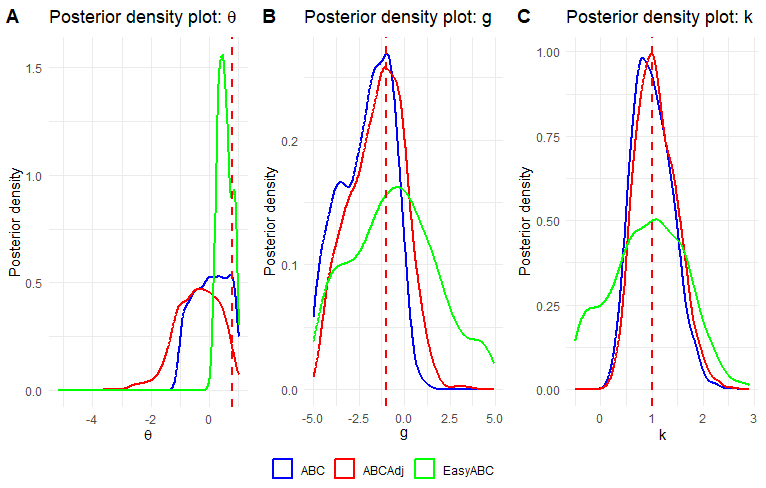
\includegraphics[width=340pt, height=200pt]{Chapters/chapter15/figures/ABCown.png}
	\caption[List of figure caption goes here]{Approximate Bayesian computation accept/reject: g-and-k distribution.}\label{figABCown}
\end{figure}

\end{enumerate}